\chapter{Results}
\label{chap:results}

There are two implemented MVDR algorithms, one assuming uniform microphone directivity and one including the directivities of the used microphones. Comparing these two gives an indication of what the influence of including the directivities are, since the directivities are the only difference between the two algorithms. It is expected that compensating for these directivities should lead to an increase in performance of the beamforming algorithm. This section covers the results of these experiments and simulations. These results are put in tables to give a clear overview of the results. 

\section{Measurement Scenario}

% \vspace{\baselineskip}
A set of experiments have been done to demonstrate the effect of the different beamformers on recorded audio. Experiments excluding and including the directivities of the microphones have been done to determine the impact including directivities has on the beamforming algorithms. In this research, the DSB, the MVDR beamformer excluding directivities and the MVDR beamformer including directivities have been investigated. 

There are two kinds of experiments conducted. The first are measurements were done in the anechoic chamber in the applied physics building at TU Delft. The other experiments are performed in an office room with dimensions $6.60m$ x $3.90m$ x $3.15m$, $[x,y,z]$.


\subsection{Anechoic Chamber experiments}

Measurements have been done in the anechoic chamber to measure recorded audio without the presence of reverberations. Two Speakers and three smartphones were used during these measurements, as illustrated in figure \ref{fig:anechoic_setup}. In this figure, the distances between the different objects are given.

\begin{figure}[h!]
	\centering  
	\includegraphics[scale=1.5, clip=true, trim = 8.25cm 17cm 10cm 9.5cm] {anechoic_setup.pdf} % l b r t]
	\caption[Setup of the measurements in the anechoic room]{Anechoic setup} 
	\label{fig:anechoic_setup}
\end{figure}

Beamforming has been performed on the recorded audio to determine the performance of the beamforming algorithms in a real room without reverberations. De audio signals and spectrograms of the source, the closest microphone and the different beamforming algorithms have been plotted in \ref{fig:anechoic_results}.
\begin{figure}[h!]
	\centering  
	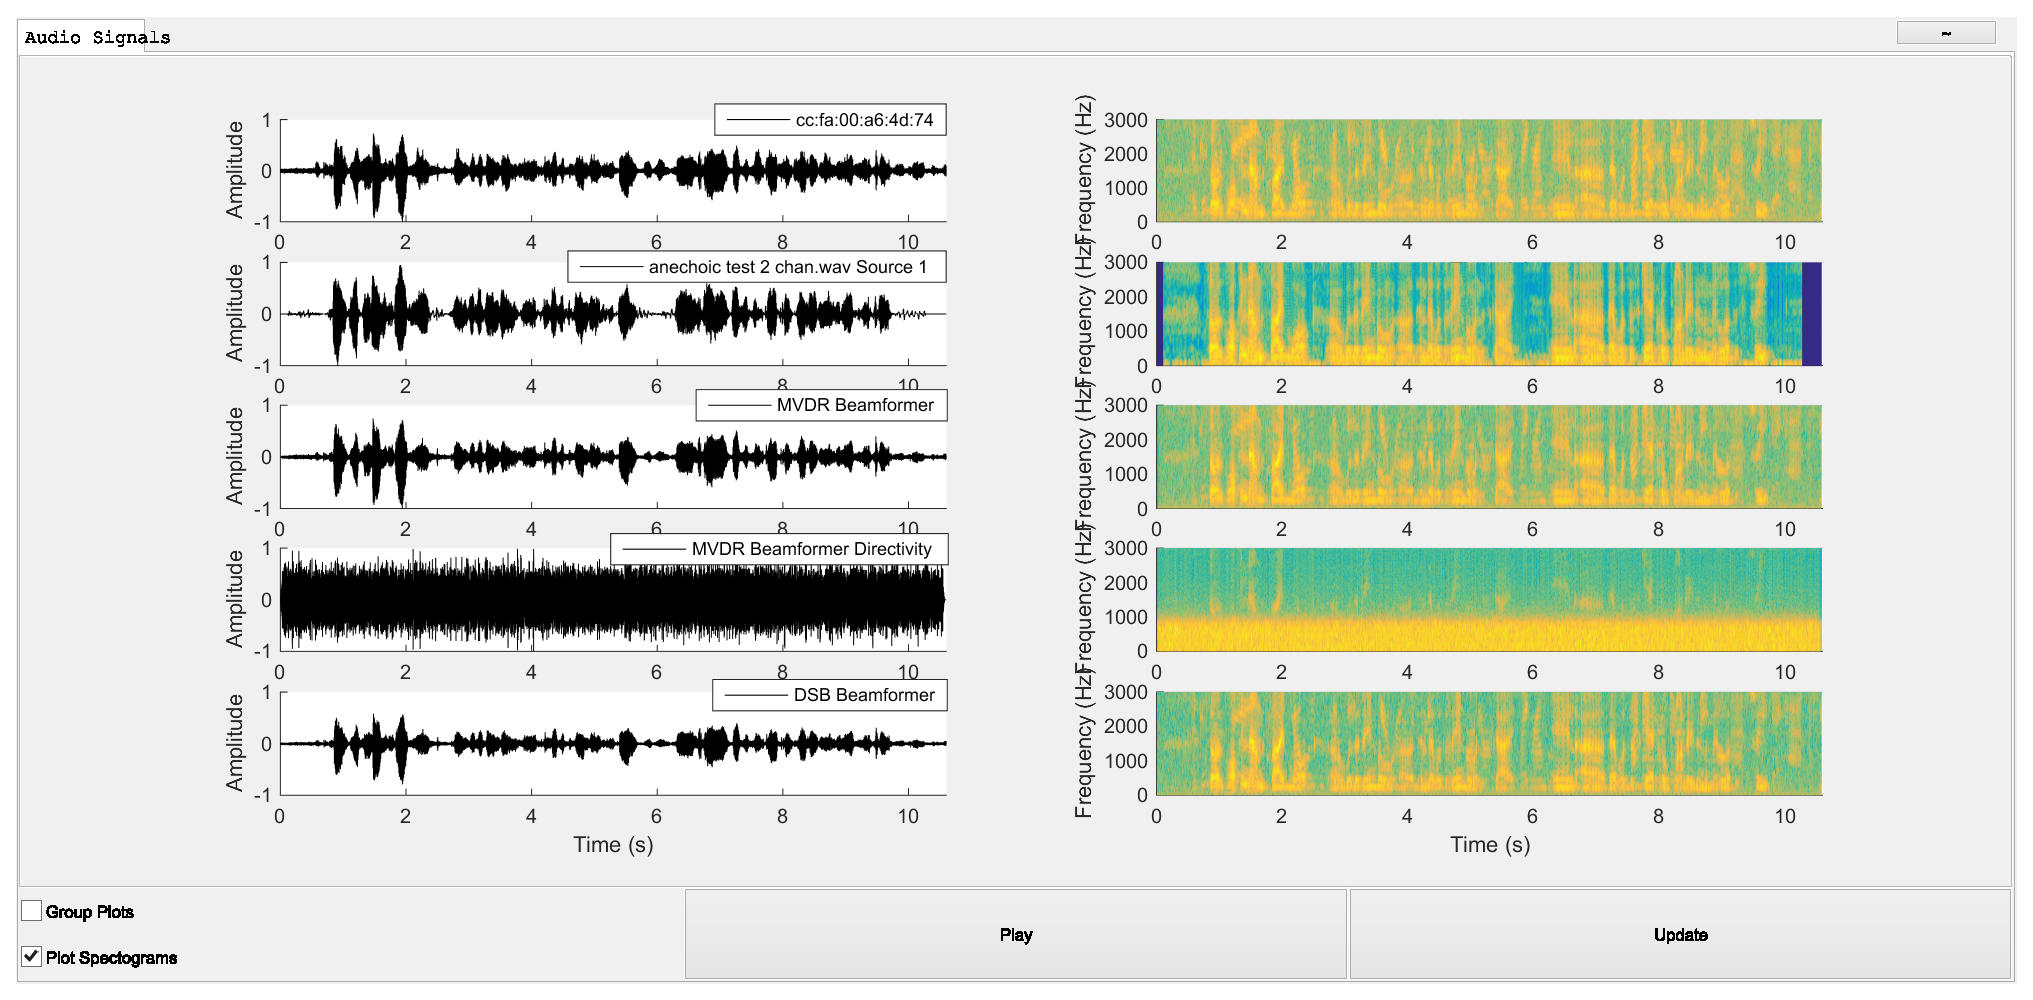
\includegraphics[width = 0.9\columnwidth] {plot_anechoic_results_with_spectogram} % l b r t]
	\caption[Audio signals and spectrogram anechoic chamber experiment 1: With an interfering audio source]{Audio signals and spectrogram anechoic chamber experiment 1: With an interfering audio source} 
	\label{fig:anechoic_results}
\end{figure}

These audio signals are used to calculate the intelligibility measures. The results of these intelligibility calculation are plotted in \ref{fig:anechoic_intelligibility} 

\begin{figure}[h!]
	\centering  
	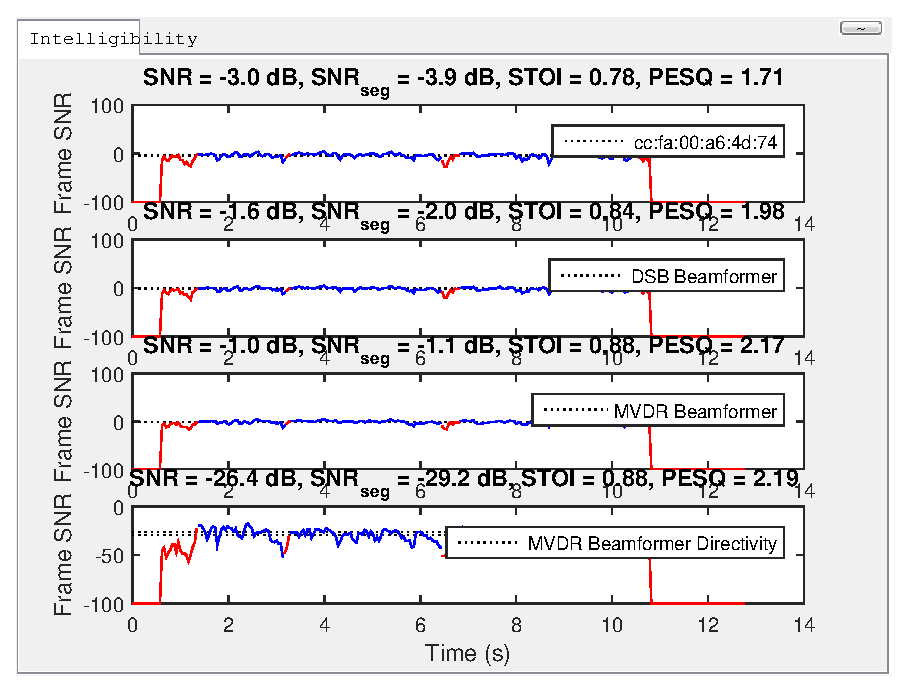
\includegraphics[width = 0.8\columnwidth] {Screenshots_experimenten/Intelligibility/anechoic} % l b r t]
	\caption[Intelligibility anechoic chamber experiment 1: With an interfering audio source]{Intelligibility anechoic chamber experiment 1: With an interfering audio source} 
	\label{fig:anechoic_intelligibility}
\end{figure}

Finally the results have been put in table \ref{tab:anechoic_res}. The results have also been put in table \ref{tab:expRes}, which is a large table at the end of the chapter with the anechoic chamber results as well as results from office room experiments. This table makes the different experimental results easily comparable.

\newpage

\begin{table}[h]
\centering
\begin{tabular}{|c|c|c|c|c|} \hline
								
								& \multicolumn{4}{c|}{Anechoic measurement} \\ \hline
								
Beamformer						& Closest  	& DSB 	& MVDR 	& MVDR+ 	\\ \hline
														
Performance measure 			&			&		&		&			\\
																						
SNR 							& -3.0		& -1.6	& -1.0	& -26.4		  \\
																						
$\text{SNR}_\text{seg}$ 		& -3.9		& -2.0	& -1.1	& -29.2		  \\
																						
STOI    						& 0.78		& 0.84	& 0.88	& 0.88		  \\
																					
PESQ  							& 1.71		& 1.98	& 2.17	& 2.19		  \\
																
White noise gain 				&			& -4.65	& 56.85	& 102.05		 \\ \hline

\end{tabular}
\caption{Experimental results of the anechoic chamber measurement}
\label{tab:anechoic_res}
\end{table}




\subsection{Office room experiments}
During the office room experiments the sound is recorded with a sampling frequency of $48000 Hz$ by smartphone microphones. This sound is used to perform the beamforming algorithms on. 

During the office room experiments, the following procedure has been followed:

\begin{itemize}
\item 2 speakers were placed at known locations with English voices, one as interference and one as source.
\item 3 smartphones placed at known locations with known orientations.
\item Both speakers played audio of english voices at the same time.
\item The smartphones streamed the audio data to the \matlab toolbox where it was recorded and synchronized.
\end{itemize}

This configuration is illustrated in figure \ref{fig:configuration}.

\begin{figure} [h!]
	\centering  
	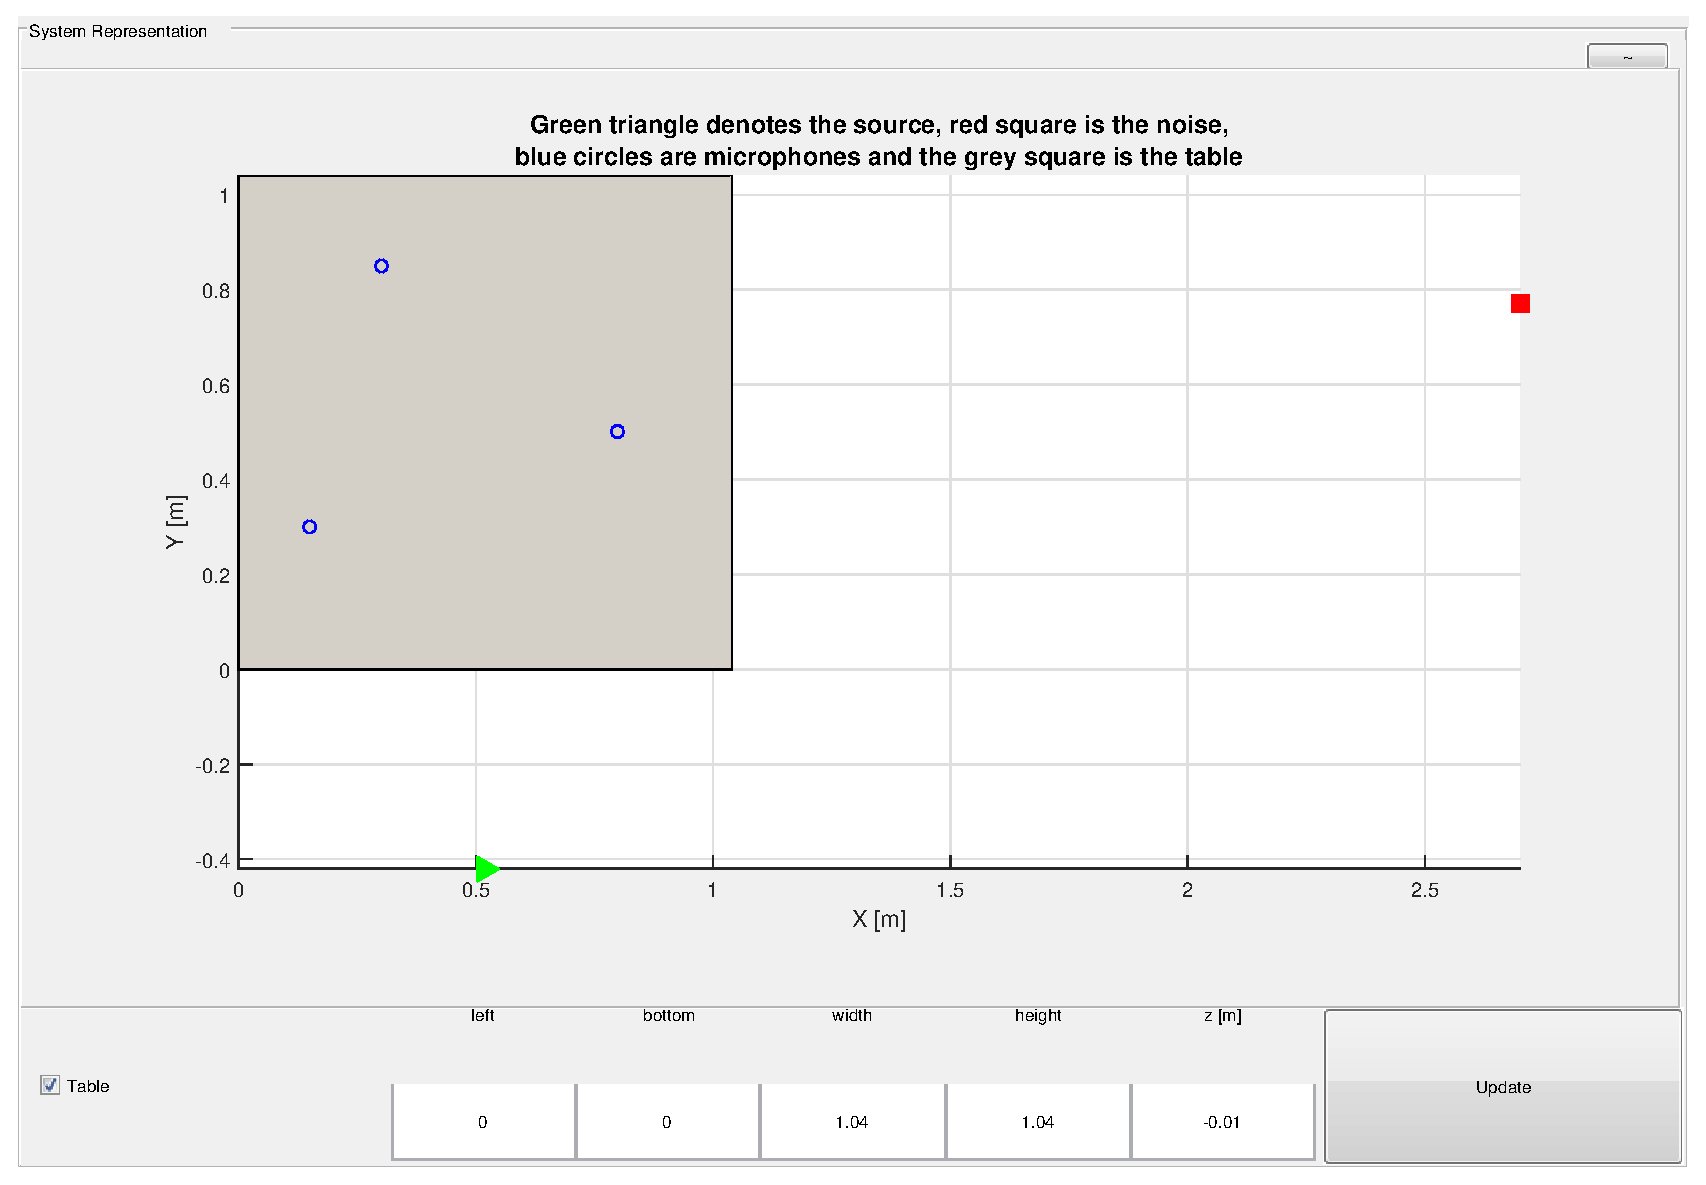
\includegraphics[scale=0.5, clip=true, trim = 2.0cm 3.5cm 1cm 1.5cm] {system_representation.eps} % l b r t]
	\caption[System configuration during the office room experiments]{Office room experiment configuration. Microphone Locations: $(0.15,0.3 , 0)$, $(0.8 , 0.5 , 0)$, $(0.3 , 0.85 , 0)$, Source Location: $(0.52 , -0.42 , 0.22)$, Interferer Location: $(2.7 , 0.77 , -0.2)$} 
	\label{fig:configuration}
\end{figure}


\subsection{Simulations of the office room experiments}

Simulations of the same microphone setup as during the office room experiments have been done to see how much the conducted experiments differ from these simulated scenario. During the simulations, the parameters as described in section \ref{sec:des_simulation} have been varied to investigate the sensitivity of the beamforming algorithms to each of the parameters. The simulated scenarios are as follows:

\newpage

\begin{table}[h!]
\centering
\begin{tabular}{|c|c|c|c|} \hline
Simulation 		& reverberations 		& Added white noise at SNR [dB] 	& Standard deviation of position errors \\ \hline
1 				& Excluded  			& 60						 		& 0 \\
2 				& Included 				& 60						 		& 0 \\
3 				& Excluded  			& 40						 		& 0 \\
4 				& Included 				& 40						 		& 0 \\
5 				& Excluded 				& 60						 		& 0.05 \\
6 				& Included  			& 60						 		& 0.05 \\ \hline
\end{tabular}
\caption{The simulated scenarios}
\label{tab:sim_scenarios}
\end{table}

A perfect match cannot be expected since the simulated microphones are omnidirectional which is not the case for smartphone microphones. However, These simulations can determine if the beamforming algorithms perform in a simulated scenario and how sensitive the beamformers are to the different parameters.

For both the DSB and MVDR beamformer, the results of the simulations are put in table \ref{tab:simRes}. For the fifth and sixth simulation, the SNR of the closest microphone has a negative value (in decibels). In this case, it is not representative for the performance of the beamformer to use the array-gain. This is because a positive SNR after a beamforming algorithm results in a negative array-gain and, in general, a negative array-gain indicates a poor performing beamforming algorithm. Therefore the entries in the table for the array gain are left blank for both these simulations.

\subsection{Results of the office room experiment}

During the conducted office room experiments, the orientation of the microphones have been varied for the microphone setup earlier illustrated in fig \ref{fig:configuration}. The investigated orientations are :

\begin{itemize}
\item $\theta = -90\degree$ (microphones facing the source)
\item $\theta = 0\degree$ (microphones facing the interfering sound source)
\item $\theta = 90\degree$ (microphones directed away from the source
\item Each microphone in a different orientation.
\end{itemize}

Where $\theta = 0\degree$ is taken in the direction of the positive x-axis and the angle increases in the counterclockwise direction. In the remainder of this section, the microphone locations are denoted by their (x,y,z) location as illustrated in figure \ref{fig:configuration}. 

A scenario with different orientations was investigated since the aim of this thesis was to research beamforming algorithms with ad-hoc microphone arrays. The orientations of the microphones in an ad-hoc microphone array will also be different for each microphone. During this experiment, the microphone located at (0.3,0.85,0) was orientated at $\theta = -90\degree$, the microphone located at (0.8,0.5,0) was orientated at $\theta = 0\degree$ and the microphone located at (0.15,0.3,0) was oriented $\theta = 90\degree$. 

The last office room experiment that has been conducted was with a linear array to compare the results of this array to the earlier ad-hoc arrays. The different microphones were located at different  with the same y-coordinate. To be exact, the locations of the microphones were (0.27,0.75,0), (0.52,0.75,0), (0.77,0.75,0).

The office room experiments were once conducted with only the source speaker playing an English voice and once with the source speaker and noise speaker playing English voices. The different performance measures as presented in section \ref{sec:des_evaluation} are calculated for each of the three beamforming algorithms and for the closest microphone. The performance measures of the closest microphone will be used to determine if and how much the signal is enhanced by the beamforming algorithms. With these results it is also possible to compare the result of each beamformimg algorithm and conclude which beamforming algorithm has the best performance. The results of the office room experiments are put in table \ref{tab:expRes}. In this table, MVDR is the standard MVDR algorithm and MVDR+ stands for the MVDR beamforming algorithm with the compensation for the directional gain of the microphones included. The SNR of the closest microphones in each of the cases is negative (in decibels) and therefore the array-gain will not give a good indication about the performance of the beamforming algorithms. For this reason, the array-gain is left out of this table.



% Simulated results
\begin{sidewaystable}[h]
\centering

\caption{Simulated results}
\label{tab:simRes}
  \begin{adjustbox}{max width=\textwidth}
\begin{tabular}{|c|c|c|c|c|c|c|c|c|c|c|c|c|c|c|c|c|}
\hline
%\multicolumn{10}{|c|}{\multirow{2}{*}{With an interfering audio source}} \\ 
%\multicolumn{10}{|l|}{} \\ \hline

 & \multicolumn{3}{c|}{Simulation 1}					& \multicolumn{3}{c|}{Simulation 2} 					& \multicolumn{3}{c|}{Simulation 3} 					\\ 
 & \multicolumn{3}{c|}{Without reverberations}			& \multicolumn{3}{c|}{With reverberations} 				& \multicolumn{3}{c|}{Without reverberations} 			\\ 
 & \multicolumn{3}{c|}{White noise added at 60dB SNR}	& \multicolumn{3}{c|}{White noise added at 60dB SNR} 	& \multicolumn{3}{c|}{White noise added at 40dB SNR} 	\\
 & \multicolumn{3}{c|}{Without position errors}			& \multicolumn{3}{c|}{Without position errors}			& \multicolumn{3}{c|}{Without position errors} 			\\ \hline
 
Beamformer				& Closest  	& DSB 		& MVDR 	& Closest  	& DSB 	& MVDR 	& Closest  	& DSB 	& MVDR \\ \hline

Performance measure 	& 	 		& 	 		& 	 	& 	 	& 		& 		&     &   	 & \\

SNR 					& 6.2		& 12.6		& 34.7 	& 2.9 	& 8.2 	& 8.6 	& 5.2 & 11.6 & 17.1 \\

$\text{SNR}_\text{seg}$	& 4.8		& 10.1		& 28.7 	& -1.3 	& 3.5 	& 5.6 	& 1.5 & 7.5 & 11.4 \\

STOI    				& 0.80		& 0.90		& 0.99 	& 0.77 	& 0.88 	& 0.95 	& 0.78 & 0.89 & 0.93 \\

PESQ  					& 1.82		& 2.29		& 3.66 	& 1.83 	& 2.16 	& 2.92 	& 1.65 & 2.09 & 2.28 \\

Array gain  			& 			& 2.03		& 5.61 	&  		& 2.78 	& 2.93 	& 	 	& 2.22 & 3.27 \\

White noise gain 		& 			& -4.64		& 51.92 & 	 	& -4.64 & 52.69 & 	 	& -4.64 & 50.94  \\ \hline \hline




 & \multicolumn{3}{c|}{Simulation 4} & \multicolumn{3}{c|}{Simulation 5} & \multicolumn{3}{c|}{Simulation 6} \\
 & \multicolumn{3}{c|}{With reverberations}				& \multicolumn{3}{c|}{Without reverberations} 						& \multicolumn{3}{c|}{With reverberations} 									\\ 
 & \multicolumn{3}{c|}{White noise added at 40dB SNR}	& \multicolumn{3}{c|}{White noise added at 60dB SNR} 				& \multicolumn{3}{c|}{White noise added at 60dB SNR} 						\\
 & \multicolumn{3}{c|}{Without position errors}			& \multicolumn{3}{c|}{with position errors with a sigma of 0.05}	& \multicolumn{3}{c|}{with position errors with a sigma of 0.05} 			\\ \hline
 
Beamformer				& Closest  	& DSB 	& MVDR 	& Closest  	& DSB 	& MVDR 	& Closest  	& DSB 	& MVDR \\ \hline

Performance measure 	& 			& 		&  		&  			&  		&  		&  			&  		& 		\\
						
SNR 					& 2.5		& 7.8	& 9.5 	& -2.4 		& 1.6 	& -2.3 	& -3.3 		& -0.1 	&  -0.6 \\
							
$\text{SNR}_\text{seg}$	& -2.1		& 3.0	& 4.9 	& -6.3 		& -3.0	& -6.5 	& -7.3 		& -4.5 	&  -3.3 \\
							
STOI    				& 0.75		& 0.87	& 0.91	& 0.68 		& 0.79 	& 0.85 	& 0.70 		& 0.76 	& 0.86 \\
							
PESQ  					& 1.66		& 2.00	& 2.25 	& 1.55 		& 1.91 	& 2.41 	& 1.75 		& 1.71 	& 2.50 \\
							
Array gain  			& 			& 3.19	& 3.88 	&  			& -0.64	& 0.94	&  			& 		&  		\\
							
White noise gain 		& 			& -4.64	& 50.96	&  			& -4.63	& 50.93	&  			& -4.64 & 51.05 \\


\hline
\end{tabular}
\end{adjustbox}
\end{sidewaystable}







% Experimental results
\begin{sidewaystable}[h]
\centering

\caption{Experimental results}
\label{tab:expRes}
  \begin{adjustbox}{max width=\textwidth}
\begin{tabular}{|c|c|c|c|c|c|c|c|c|c|c|c|c|c|c|c|c|}
\hline
\multicolumn{13}{|c|}{\multirow{2}{*}{Without an interfering audio source}} \\ 
\multicolumn{13}{|c|}{} \\ \hline

						& \multicolumn{4}{c|}{$\theta = -90\degree$}	& \multicolumn{4}{c|}{$\theta = 0\degree$} 	& \multicolumn{4}{c|}{$\theta = -90\degree$} \\ \hline
	
Beamformer				& Closest  	& DSB 	& MVDR 	& MVDR+ 		& Closest  	& DSB 	& MVDR 	& MVDR+ 		& Closest  	& DSB 	& MVDR 	& MVDR+ \\ \hline
				
Performance measure 	& 			& 		&   	&   			& 	 		&   	& 	 	&   			& 			& 		&  		&  \\
				
SNR 					& -6.5		& -5.9	& -9.4 	& -32.1 		& -6.7 		& -6.2 	& -14.3 & -47.3 		& -6.5		& -5.8	& -9.5 	& -33.3 \\
						
$\text{SNR}_\text{seg}$	& -3.0		& -1.8	& -6.4 	& -31.7 		& -7.0 		& -6.0 	& -15.5 & -49.9 		& -6.6		& -5.4	& -10.7	& -35.9 \\
						
STOI   					& 0.73		& 0.81	& 0.73	& 0.74 			& 0.71 		& 0.76 	& 0.50 	& 0.51  		& 0.71		& 0.76	& 0.58 	& 0.57 	\\
						
PESQ  					& 2.45		& 2.68	& 2.18 	& 2.24 			& 2.34 		& 2.53 	& 1.47 	& 1.55  		& 2.36		& 2.54	& 1.78 	& 1.74	\\
						
White noise gain 		& 			& -4.64	& 50.99 & 105.06 		&   		& -4.63 & 52.24 & 96.59 		& 			& -4.64	& 52.21 & 93.80 \\ \hline

						& \multicolumn{4}{c|}{Different orientations}& \multicolumn{4}{c|}{Linear array}  		\\ \cline{1-9}

Beamformer				& Closest  	& DSB 	& MVDR 	& MVDR+ 		& Closest  	& DSB 	& MVDR 		& MVDR+ 	\\ \cline{1-9}
	
Performance measure 	&  			&  		&  		&  				&  			&  		&  			&  			\\
	
SNR 					& -6.4 		& -5.8 	& -9.8 	& -34.7 		& -7.1 		& -8.6 	& -13.0 	& -55.3 	\\
									
$\text{SNR}_\text{seg}$	& -6.3 		& -5.2 	& -10.8 & -37.3 		& -7.0 		& -11.0 & -14.1 	& -57.9 	\\
			
STOI    				& 0.70 		& 0.78 	& 0.58 	& 0.58 			& -13.0 	& 0.51 	& 0.47 		& 0.48 		\\
										
PESQ  					& 2.36 		& 2.59 	& 1.71 	& 1.74 			& -55.3 	& 2.04 	& 1.53 		& 1.70 		\\
	
White noise gain 		&  			& -4.64 & 52.66 & 96.19 		&  			& -4.77 & 54.08 	& 105.10 	\\

\hline \hline 
\multicolumn{13}{|c|}{\multirow{2}{*}{With an interfering audio source}} \\ 
\multicolumn{13}{|l|}{} \\ \hline

						& \multicolumn{4}{c|}{$\theta = -90\degree$} 	& \multicolumn{4}{c|}{$\theta = 0\degree$} 	& \multicolumn{4}{c|}{$\theta = 90\degree$} \\ \hline

Beamformer				& Closest  	& DSB 	& MVDR 	& MVDR+ 		& Closest  	& DSB 	& MVDR 	& MVDR+ 		& Closest  	& DSB 	& MVDR 	& MVDR+  \\ \hline

Performance measure 	& 			& 		&  		&  				&  			&  		&  		&  				&	  		&  		&  		& \\ 

SNR 					& -6.8 & -5.8 & -7.0 & -29.9 & -7.3 & -6.3 & -8.9 & -31.2 & -6.7	& -6.5	& -13.8 & -53 \\ 

$\text{SNR}_\text{seg}$	& -6.7 & -5.0 & -7.8 & -32.5 & -7.8 & -6.1 & -9.7 & -33.8 & -7.3	& -7.6	& -15.7 & -55.6 \\

STOI    				& 0.70 & 0.79 & 0.64 & 0.65 & 0.66 & 0.72 & 0.56 & 0.58 & 0.65	& 0.65	& 0.48 & 0.47 	\\

PESQ  					& 2.32 & 2.54 & 1.81 & 1.89 & 2.10 & 2.37 & 1.72 & 1.83 & 2.06	& 1.97	& 1.29 & 1.39 	\\

White noise gain 		&  	  & -4.64 & 52.82 & 105.08 &   & -4.64 & 52.33 & 96.53 &  		& -4.64	& 51.96 & 93.82 \\ \hline

						& \multicolumn{4}{c|}{Different orientations}& \multicolumn{4}{c|}{Linear array} 	& \multicolumn{4}{c|}{Anechoic measurement} \\ \hline

Beamformer				& Closest  	& DSB 	& MVDR 	& MVDR+ 		& Closest  	& DSB 	& MVDR 	& MVDR+ 	& Closest  	& DSB 	& MVDR 	& MVDR+ 	\\ \hline

Performance measure 	&  			&  		&  		&  				&  			&  		&  		&  			&			&		&		&			\\

SNR 					& -6.8		& -6.0 	& -7.9 	& -28.5 		& -7.1		& -6.2	& -7.2 	& -34.1 	& -3.0		& -1.6	& -1.0	& -26.4		  \\
								
$\text{SNR}_\text{seg}$ & -7.5		& -5.9 	& -8.8 	& -31.1 		& -7.6		& -6.2	& -8.1 	& -36.7 	& -3.9		& -2.0	& -1.1	& -29.2		  \\
								
STOI    				& 0.64		& 0.73 	& 0.58 	& 0.60 			& 0.67		& 0.70	& 0.53 	& 0.54 		& 0.78		& 0.84	& 0.88	& 0.88		  \\
								
PESQ  					& 2.08		& 2.36 	& 1.72 	& 1.81 			& 2.12 		& 2.30	& 1.68 	& 1.80 		& 1.71		& 1.98	& 2.17	& 2.19		  \\
					
White noise gain 		& 			& -4.64 & 52.24 & 98.88 		&  			& -4.77 & 54.56 & 104.99  	&			& -4.65	& 56.85	& 102.05		 \\

\hline
\end{tabular}
\end{adjustbox}
\end{sidewaystable}





% Oude tabellen

%\begin{figure} [h!]
%	\minipage{0.32\textwidth}
%		\fbox{\includegraphics[width = \linewidth, clip=true, trim = 9.75cm 3.25cm 		9.0cm 1.1cm] {mic_array_example}} % l b r t]
%		\caption{EXAMPLE Microphone setup A} 
%		\label{fig:arrayA}
%	\endminipage \hfill
%	\minipage{0.32\textwidth}
%		\fbox{\includegraphics[width = \linewidth, clip=true, trim = 9.75cm 3.25cm 		9.0cm 1.1cm] {mic_array_example}} % l b r t]
%		\caption{EXAMPLE Microphone setup B} 
%		\label{fig:arrayB}
%	\endminipage \hfill
%	\minipage{0.32\textwidth}
%		\fbox{\includegraphics[width = \linewidth, clip=true, trim = 9.75cm 3.25cm 		9.0cm 1.1cm] {mic_array_example}} % l b r t]
%		\caption{EXAMPLE Microphone setup C} 
%		\label{fig:arrayC}
%	\endminipage%
%\end{figure}

%\begin{figure}
%\centering
%\begin{subfigure}{.5\textwidth}
%  \centering
%  \includegraphics[width = \linewidth, clip=true, trim = 9.75cm 3.25cm 		9.0cm 1.1cm] {mic_array_example}
%  \caption{EXAMPLE Microphone setup A}
%  \label{fig:arrayA}
%\end{subfigure}%
%\begin{subfigure}{.5\textwidth}
%  \centering
%  \includegraphics[width = \linewidth, clip=true, trim = 9.75cm 3.25cm 		9.0cm 1.1cm] {mic_array_example}
%  \caption{EXAMPLE Microphone setup B}
%  \label{fig:arrayB}
%\end{subfigure}
%\caption[Microphone setups used during the experiments] {A figure with two subfigures}
%\label{fig:test}
%\end{figure}



%\vspace{\baselineskip}
%{\Huge Possible tables:} \\
%\vspace{\baselineskip}
%\begin{tabular}{|c|c|c|c|c|c|c|}
%\hline 
%• & SNR & SNR seg & WNG & Array Gain & STOI & PESQ \\ 
%\hline 
%Closest Mic & • & • & • & • & • & • \\ 
%\hline 
%DSB & • & • & • & • & • & • \\ 
%\hline 
%MVDR & • & • & • & • & • & • \\ 
%\hline 
%MVDR+ & • & • & • & • & • & • \\ 
%\hline 
%\end{tabular}
%\vspace{\baselineskip}
%Or \\
%\vspace{\baselineskip}
%
%\textit{FOR EXAMPLE}
%The segmental SNR for the different microphone arrays:
%
%\begin{tabular}{|c|c|c|c|c|c|c|}
%\hline 
%Microphone array & Closest Mic & DSB & MVDR & MVDR+ \\ 
%\hline 
%A & • & • & • & • \\ 
%\hline 
%B & • & • & • & • \\ 
%\hline 
%C & • & • & • & • \\ 
%\hline 
%D & • & • & • & • \\ 
%\hline 
%\end{tabular}

%\vspace{\baselineskip}
%
%\begin{sidewaystable}[h]
%\centering
%
%\caption[Experimental results belonging to microphone array A]{Microphone array A}
%\label{tab:resultsA}
%  \begin{adjustbox}{max width=\textwidth}
%\begin{tabular}{|c|c|c|c|c|c|c|c|c|c|c|c|c|c|c|c|c|}
%\hline
%Beamformer 	& \multicolumn{4}{c|}{Simulation} 	& \multicolumn{4}{c|}{$\theta$ = theta1} & \multicolumn{4}{c|}{$\theta$ = theta2} & \multicolumn{4}{c|}{$\theta$ = theta3} \\ \hline
%Performance measure & SNR & $\text{SNR}_\text{seg}$ & STOI & PESQ &	& &	& &	& & & & & & & \\ \hline
%Closest 	& 	$SNR$ Simulation	& $SNR_{seg}$ Simulation& $STOI$ Simulation & $PESQ$ Simulation 	& $SNR$ theta1 & $SNR_{seg}$ theta1 & $STOI$ theta1 & $PESQ$ theta1								& 	$SNR$ theta2		& $SNR_{seg}$ theta2	& $STOI$ theta2 	& $PESQ$ theta2			& $SNR$ theta3 & $SNR_{seg}$ theta3	& $STOI$ theta3	& $PESQ$ theta3 \\
%DSB 		& 	$SNR$ Simulation	& $SNR_{seg}$ Simulation& $STOI$ Simulation & $PESQ$ Simulation 	& $SNR$ theta1 & $SNR_{seg}$ theta1 & $STOI$ theta1 & $PESQ$ theta1								& 	$SNR$ theta2		& $SNR_{seg}$ theta2	& $STOI$ theta2 	& $PESQ$ theta2			& $SNR$ theta3 & $SNR_{seg}$ theta3	& $STOI$ theta3	& $PESQ$ theta3 \\
%MVDR    	& 	$SNR$ Simulation	& $SNR_{seg}$ Simulation& $STOI$ Simulation & $PESQ$ Simulation 	& $SNR$ theta1 & $SNR_{seg}$ theta1 & $STOI$ theta1 & $PESQ$ theta1								& 	$SNR$ theta2		& $SNR_{seg}$ theta2	& $STOI$ theta2 	& $PESQ$ theta2			& $SNR$ theta3 & $SNR_{seg}$ theta3	& $STOI$ theta3	& $PESQ$ theta3 \\
%MVDR+  		& 	$SNR$ Simulation	& $SNR_{seg}$ Simulation& $STOI$ Simulation & $PESQ$ Simulation 	& $SNR$ theta1 & $SNR_{seg}$ theta1 & $STOI$ theta1 & $PESQ$ theta1								& 	$SNR$ theta2		& $SNR_{seg}$ theta2	& $STOI$ theta2 	& $PESQ$ theta2			& $SNR$ theta3 & $SNR_{seg}$ theta3	& $STOI$ theta3	& $PESQ$ theta3 \\ \hline
%\end{tabular}
%\end{adjustbox}
%
%\vspace{\baselineskip}
%
%\caption[Experimental results belonging to microphone array B]{Microphone array B}
%\label{tab:resultsB}
%  \begin{adjustbox}{max width=\textwidth}
%\begin{tabular}{|l|l|l|l|l|l|l|l|l|l|l|l|l|l|l|l|l|}
%\hline
%Beamformer 	& \multicolumn{4}{c|}{Simulation} 	& \multicolumn{4}{c|}{$\theta$ = theta1} & \multicolumn{4}{c|}{$\theta$ = theta2} & \multicolumn{4}{c|}{$\theta$ = theta3} \\ \hline
% & & & & &	& &	& &	& & & & & & & \\
%Closest 	& 	$SNR$ Simulation	& $SNR_{seg}$ Simulation& $STOI$ Simulation & $PESQ$ Simulation 	& $SNR$ theta1 & $SNR_{seg}$ theta1 & $STOI$ theta1 & $PESQ$ theta1								& 	$SNR$ theta2		& $SNR_{seg}$ theta2	& $STOI$ theta2 	& $PESQ$ theta2			& $SNR$ theta3 & $SNR_{seg}$ theta3	& $STOI$ theta3	& $PESQ$ theta3 \\
%DSB 		& 	$SNR$ Simulation	& $SNR_{seg}$ Simulation& $STOI$ Simulation & $PESQ$ Simulation 	& $SNR$ theta1 & $SNR_{seg}$ theta1 & $STOI$ theta1 & $PESQ$ theta1								& 	$SNR$ theta2		& $SNR_{seg}$ theta2	& $STOI$ theta2 	& $PESQ$ theta2			& $SNR$ theta3 & $SNR_{seg}$ theta3	& $STOI$ theta3	& $PESQ$ theta3 \\
%MVDR    	& 	$SNR$ Simulation	& $SNR_{seg}$ Simulation& $STOI$ Simulation & $PESQ$ Simulation 	& $SNR$ theta1 & $SNR_{seg}$ theta1 & $STOI$ theta1 & $PESQ$ theta1								& 	$SNR$ theta2		& $SNR_{seg}$ theta2	& $STOI$ theta2 	& $PESQ$ theta2			& $SNR$ theta3 & $SNR_{seg}$ theta3	& $STOI$ theta3	& $PESQ$ theta3 \\
%MVDR+  		& 	$SNR$ Simulation	& $SNR_{seg}$ Simulation& $STOI$ Simulation & $PESQ$ Simulation 	& $SNR$ theta1 & $SNR_{seg}$ theta1 & $STOI$ theta1 & $PESQ$ theta1								& 	$SNR$ theta2		& $SNR_{seg}$ theta2	& $STOI$ theta2 	& $PESQ$ theta2			& $SNR$ theta3 & $SNR_{seg}$ theta3	& $STOI$ theta3	& $PESQ$ theta3 \\ \hline
%\end{tabular}
%\end{adjustbox}
%
%\vspace{\baselineskip}
%
%\caption[Experimental results belonging to microphone array C]{Microphone array C}
%\label{tab:resultsC}
%  \begin{adjustbox}{max width=\textwidth}
%\begin{tabular}{|l|l|l|l|l|l|l|l|l|l|l|l|l|l|l|l|l|}
%\hline
%Beamformer 	& \multicolumn{4}{c|}{Simulation} 	& \multicolumn{4}{c|}{$\theta$ = theta1} & \multicolumn{4}{c|}{$\theta$ = theta2} & \multicolumn{4}{c|}{$\theta$ = theta3} \\ \hline
% & & & & &	& &	& &	& & & & & & & \\
%Closest 	& 	$SNR$ Simulation	& $SNR_{seg}$ Simulation& $STOI$ Simulation & $PESQ$ Simulation 	& $SNR$ theta1 & $SNR_{seg}$ theta1 & $STOI$ theta1 & $PESQ$ theta1								& 	$SNR$ theta2		& $SNR_{seg}$ theta2	& $STOI$ theta2 	& $PESQ$ theta2			& $SNR$ theta3 & $SNR_{seg}$ theta3	& $STOI$ theta3	& $PESQ$ theta3 \\
%DSB 		& 	$SNR$ Simulation	& $SNR_{seg}$ Simulation& $STOI$ Simulation & $PESQ$ Simulation 	& $SNR$ theta1 & $SNR_{seg}$ theta1 & $STOI$ theta1 & $PESQ$ theta1								& 	$SNR$ theta2		& $SNR_{seg}$ theta2	& $STOI$ theta2 	& $PESQ$ theta2			& $SNR$ theta3 & $SNR_{seg}$ theta3	& $STOI$ theta3	& $PESQ$ theta3 \\
%MVDR    	& 	$SNR$ Simulation	& $SNR_{seg}$ Simulation& $STOI$ Simulation & $PESQ$ Simulation 	& $SNR$ theta1 & $SNR_{seg}$ theta1 & $STOI$ theta1 & $PESQ$ theta1								& 	$SNR$ theta2		& $SNR_{seg}$ theta2	& $STOI$ theta2 	& $PESQ$ theta2			& $SNR$ theta3 & $SNR_{seg}$ theta3	& $STOI$ theta3	& $PESQ$ theta3 \\
%MVDR+  		& 	$SNR$ Simulation	& $SNR_{seg}$ Simulation& $STOI$ Simulation & $PESQ$ Simulation 	& $SNR$ theta1 & $SNR_{seg}$ theta1 & $STOI$ theta1 & $PESQ$ theta1								& 	$SNR$ theta2		& $SNR_{seg}$ theta2	& $STOI$ theta2 	& $PESQ$ theta2			& $SNR$ theta3 & $SNR_{seg}$ theta3	& $STOI$ theta3	& $PESQ$ theta3 \\ \hline
%\end{tabular}
%\end{adjustbox}
%\end{sidewaystable}

%\begin{sidewaystable}[h]
%\centering
%
%\caption[]{Experimental results including interference}
%\label{tab:resultsA}
%  \begin{adjustbox}{max width=\textwidth}
%\begin{tabular}{|c|c|c|c|c|c|c|c|c|c|c|c|c|c|c|c|c|}
%\hline
%• & \multicolumn{4}{c|}{Simulation}	& \multicolumn{4}{c|}{$\theta$ = theta1} & \multicolumn{4}{c|}{$\theta$ = theta2}  \\ \hline
%
%Beamformer				& Closest  	& DSB 	& MVDR 	& MVDR+ & Closest  	& DSB 	& MVDR 	& MVDR+ & Closest  	& DSB 	& MVDR 	& MVDR+ \\ \hline
%
%Performance measure 	& •	& •& • & • & • & • & • & • & • & • & • & •  \\
%
%$SNR$ 					& •	& •& • & • & -6.8 & -5.8 & -7.0 & -29.9 & -7.3 & -6.3 & -8.9 & -31.2  \\
%
%$SNR_{seg}$ 			& •	& •& • & • & -6.7 & -5.0 & -7.8 & -32.5 & -7.8 & -6.1 & -9.7 & -33.8 \\
%
%$STOI$    				& •	& •& • & • & 0.70 & 0.79 & 0.64 & 0.65 & 0.66 & 0.72 & 0.56 & 0.58 \\
%
%$PESQ$  				& •	& •& • & • & 2.32 & 2.54 & 1.81 & 1.89 & 2.10 & 2.37 & 1.72 & 1.83 \\
%
%$Array gain$  			& •	& •& • & • &      & 0.86 & 1.03 & 4.39 & 	  & 0.86 & 1.22 & 4.25 \\
%
%$White noise gain$ 		& •	& •& • & • &  	  & -4.64 & 52.82 & 105.08 &   & -4.64 & 52.33 & 96.53 \\ \hline
%
%• & \multicolumn{4}{c|}{$\theta$ = theta3} & \multicolumn{4}{c|}{$\theta$ = theta4} & \multicolumn{4}{c|}{Linear array} \\ \hline
%
%Beamformer				& Closest  	& DSB 	& MVDR 	& MVDR+ & Closest  	& DSB 	& MVDR 	& MVDR+ & Closest  	& DSB 	& MVDR 	& MVDR+ \\ \hline
%
%Performance measure 	& •	& •& • & • & • & • & • & • & • & • & • & •  \\
%
%$SNR$ 					& -6.7	& -6.5	& -13.8 & -53 	& -6.8	& -6.0 & -7.9 & -28.5 & -7.1	& -6.2& -7.2 & -34.1   \\
%
%$SNR_{seg}$ 			& -7.3	& -7.6	& -15.7 & -55.6 & -7.5	& -5.9 & -8.8 & -31.1 & -7.6	& -6.2& -8.1 & -36.7   \\
%
%$STOI$    				& 0.65	& 0.65	& 0.48 & 0.47 	& 0.64	& 0.73 & 0.58 & 0.60 & 0.67		& 0.70& 0.53 & 0.54   \\
%
%$PESQ$  				& 2.06	& 1.97	& 1.29 & 1.39 	& 2.08	& 2.36 & 1.72 & 1.81 & 2.12 	& 2.30& 1.68 & 1.80   \\
%
%$Array gain$  			&  		& 0.96 	& 2.05 & 7.86 	& 		& 0.88	& 1.16 & 4.20 &  		& 0.86& 1.01 & 4.78   \\
%
%$White noise gain$ 		&  		& -4.64	& 51.96 & 93.82 & 		& -4.64 & 52.24 & 98.88 &  		& -4.77 & 54.56 & 104.99   \\
%
%
%\end{tabular}
%\end{adjustbox}
%\end{sidewaystable}






%\hline \hline 
%\multicolumn{13}{|c|}{\multirow{2}{*}{With an interfering audio source}} \\ 
%\multicolumn{13}{|l|}{} \\ \hline
%
%• & \multicolumn{4}{c|}{Simulation}	& \multicolumn{4}{c|}{$\theta$ = theta1} & \multicolumn{4}{c|}{$\theta$ = theta2}  \\ \hline
%
%Beamformer				& Closest  	& DSB 	& MVDR 	& MVDR+ & Closest  	& DSB 	& MVDR 	& MVDR+ & Closest  	& DSB 	& MVDR 	& MVDR+ \\ \hline
%
%Performance measure 	& •	& •& • & • & • & • & • & • & • & • & • & •  \\
%
%$SNR$ 					& •	& •& • & • & -6.8 & -5.8 & -7.0 & -29.9 & -7.3 & -6.3 & -8.9 & -31.2  \\
%
%$SNR_{seg}$ 			& •	& •& • & • & -6.7 & -5.0 & -7.8 & -32.5 & -7.8 & -6.1 & -9.7 & -33.8 \\
%
%$STOI$    				& •	& •& • & • & 0.70 & 0.79 & 0.64 & 0.65 & 0.66 & 0.72 & 0.56 & 0.58 \\
%
%$PESQ$  				& •	& •& • & • & 2.32 & 2.54 & 1.81 & 1.89 & 2.10 & 2.37 & 1.72 & 1.83 \\
%
%$Array gain$  			& •	& •& • & • &      & 0.86 & 1.03 & 4.39 & 	  & 0.86 & 1.22 & 4.25 \\
%
%$White noise gain$ 		& •	& •& • & • &  	  & -4.64 & 52.82 & 105.08 &   & -4.64 & 52.33 & 96.53 \\ \hline
%
%• & \multicolumn{4}{c|}{$\theta$ = theta3} & \multicolumn{4}{c|}{$\theta$ = theta4} & \multicolumn{4}{c|}{Linear array} \\ \hline
%
%Beamformer				& Closest  	& DSB 	& MVDR 	& MVDR+ & Closest  	& DSB 	& MVDR 	& MVDR+ & Closest  	& DSB 	& MVDR 	& MVDR+ \\ \hline
%
%Performance measure 	& •	& •& • & • & • & • & • & • & • & • & • & •  \\
%
%$SNR$ 					& -6.7	& -6.5	& -13.8 & -53 	& -6.8	& -6.0 & -7.9 & -28.5 & -7.1	& -6.2& -7.2 & -34.1   \\
%
%$SNR_{seg}$ 			& -7.3	& -7.6	& -15.7 & -55.6 & -7.5	& -5.9 & -8.8 & -31.1 & -7.6	& -6.2& -8.1 & -36.7   \\
%
%$STOI$    				& 0.65	& 0.65	& 0.48 & 0.47 	& 0.64	& 0.73 & 0.58 & 0.60 & 0.67		& 0.70& 0.53 & 0.54   \\
%
%$PESQ$  				& 2.06	& 1.97	& 1.29 & 1.39 	& 2.08	& 2.36 & 1.72 & 1.81 & 2.12 	& 2.30& 1.68 & 1.80   \\
%
%$Array gain$  			&  		& 0.96 	& 2.05 & 7.86 	& 		& 0.88	& 1.16 & 4.20 &  		& 0.86& 1.01 & 4.78   \\
%
%$White noise gain$ 	&  		& -4.64	& 51.96 & 93.82 & 		& -4.64 & 52.24 & 98.88 &  		& -4.77 & 54.56 & 104.99   \\